\paragraph{LLGS form with field-like torque.}
This macrospin equation is adapted from Eqs.~(1)--(4) of Kong et al., with the
atom index removed~\cite{kong2026spatially}.  It is written in the
flux-density convention: $\vect{B}_{\mathrm{eff}}$ and the torque amplitudes
are in tesla and are paired with $\gamma$ in
$\mathrm{rad\,s^{-1}\,T^{-1}}$.
\begin{align}
    \frac{\dd\mvec}{\dd t}
    ={}& -\gamma\,\mvec\times\vect{B}_{\mathrm{eff}}
         + \alpha\,\mvec\times\frac{\dd\mvec}{\dd t}
         - \gamma\tau_{\mathrm{DLT}}\,
           \mvec\times\bigl(\mvec\times\vect{\sigma}\bigr)
         \notag\\
       & + \gamma\tau_{\mathrm{FLT}}\,
           \mvec\times\vect{\sigma}.
    \label{eq:llg-gilbert}
\end{align}

Figure~\ref{fig:sot-llgs-geometry} fixes the device axes and illustrates the
vector structures that appear in Eq.~\eqref{eq:llg-gilbert}.

\begin{figure}[htbp]
    \centering
    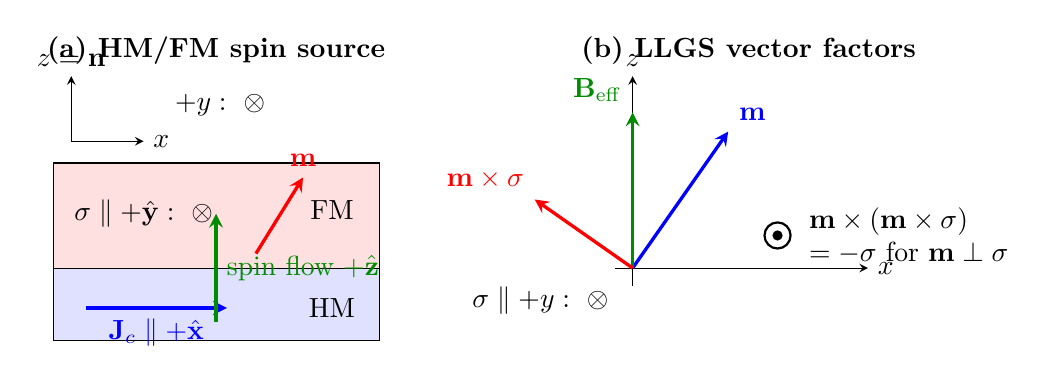
\begin{tikzpicture}[>=stealth,scale=0.92]
        \begin{scope}
            \node[font=\bfseries] at (2.25,3.0)
                {(a) HM/FM spin source};
            \draw[fill=blue!12] (0,-1.0) rectangle (4.5,0);
            \draw[fill=red!12] (0,0) rectangle (4.5,1.45);
            \node at (3.85,-0.55) {HM};
            \node at (3.85,0.8) {FM};

            \draw[->,very thick,blue] (0.45,-0.55) -- (2.4,-0.55)
                node[midway,below] {$\mathbf J_c\parallel+\hat{\mathbf x}$};
            \draw[->,very thick,green!55!black] (2.25,-0.75) -- (2.25,0.75)
                node[midway,right] {spin flow $+\hat{\mathbf z}$};
            \node at (1.25,0.75) {$\boldsymbol{\sigma}\parallel+\hat{\mathbf y}:\ \otimes$};
            \draw[->,very thick,red] (2.8,0.2) -- (3.45,1.25)
                node[above] {$\mathbf m$};

            \draw[->] (0.25,1.75) -- (1.25,1.75) node[right] {$x$};
            \draw[->] (0.25,1.75) -- (0.25,2.65) node[above] {$z=\mathbf n$};
            \node[anchor=west] at (1.55,2.25) {$+y:\ \otimes$};
        \end{scope}

        \begin{scope}[xshift=8cm]
            \node[font=\bfseries] at (1.6,3.0)
                {(b) LLGS vector factors};
            \draw[->] (-0.25,0) -- (3.25,0) node[right] {$x$};
            \draw[->] (0,-0.25) -- (0,2.65) node[above] {$z$};
            \node[anchor=east] at (-0.2,-0.45)
                {$\boldsymbol{\sigma}\parallel+y:\ \otimes$};

            \draw[->,very thick,blue] (0,0) -- (55:2.3)
                node[above right] {$\mathbf m$};
            \draw[->,very thick,green!55!black] (0,0) -- (0,2.15)
                node[above left] {$\mathbf B_{\mathrm{eff}}$};
            \draw[->,very thick,red] (0,0) -- (145:1.65)
                node[above left] {$\mathbf m\times\boldsymbol{\sigma}$};

            \draw[thick] (2.0,0.45) circle (0.18);
            \fill (2.0,0.45) circle (2pt);
            \node[align=left,anchor=west] at (2.3,0.45)
                {$\mathbf m\times(\mathbf m\times\boldsymbol{\sigma})$\\
                 $=-\boldsymbol{\sigma}$ for $\mathbf m\perp\boldsymbol{\sigma}$};
        \end{scope}
    \end{tikzpicture}
    \caption{Original schematic of a conventional spin-Hall-driven LLGS
    geometry.  (a) Charge current along $+x$ in the heavy metal generates a
    spin flow along the interface normal $+z$ with the illustrated polarization
    along $+y$; reversing the current or the signed spin-Hall angle reverses the
    polarization.  (b) For $\mathbf m$ in the $xz$ plane, the field-like vector
    $\mathbf m\times\boldsymbol{\sigma}$ lies in that plane, whereas the
    damping-like vector $\mathbf m\times(\mathbf m\times\boldsymbol{\sigma})$
    points along $-y$.  These are vector factors only; their signed scalar
    prefactors are those in Eq.~\eqref{eq:llg-gilbert}.  The conventions follow
    the SOT compact model and Kong \emph{et al.}
    ~\cite{sot-stt-compact-model,kong2026spatially}.}
    \label{fig:sot-llgs-geometry}
\end{figure}

\paragraph{Equivalent LL form with field-like torque.}
The algebraically equivalent form follows the same source
convention~\cite{kong2026spatially}.
\begin{align}
    \bigl(1+\alpha^2\bigr)\frac{\dd\mvec}{\dd t}
    ={}& -\gamma\,\mvec\times\vect{B}_{\mathrm{eff}}
         - \alpha\gamma\,\mvec\times
           \bigl(\mvec\times\vect{B}_{\mathrm{eff}}\bigr)
         \notag\\
       & + \alpha\gamma\tau_{\mathrm{DLT}}\,
           \mvec\times\vect{\sigma}
         - \gamma\tau_{\mathrm{DLT}}\,
           \mvec\times\bigl(\mvec\times\vect{\sigma}\bigr)
         \notag\\
       & + \alpha\gamma\tau_{\mathrm{FLT}}\,
           \mvec\times\bigl(\mvec\times\vect{\sigma}\bigr)
         + \gamma\tau_{\mathrm{FLT}}\,
           \mvec\times\vect{\sigma}.
    \label{eq:ll-with-flt}
\end{align}

\paragraph{Torque amplitudes.}
For a ferromagnetic layer~\cite{zhang2024revisiting},
\[
    \tau_{\mathrm{DLT}}
    = \frac{\hbar\theta_{\mathrm{SH}}J_c}
           {2e\,t_{\mathrm{FM}}\Ms},
    \qquad
    \tau_{\mathrm{FLT}}
    = \beta\tau_{\mathrm{DLT}}.
\]

\paragraph{Torque-sign convention.}
In the convention of Eq.~\eqref{eq:llg-gilbert}, the sign product of the
damping-like and field-like SOT is negative when
$\beta>0$~\cite{park2014macrospin,kong2026spatially}.  Specifically, the
scalar prefactors of their respective vector structures are
$-\gamma\tau_{\mathrm{DLT}}$ and $+\gamma\tau_{\mathrm{FLT}}$, so their sign
product is
\[
    \bigl(-\gamma\tau_{\mathrm{DLT}}\bigr)
    \bigl(+\gamma\tau_{\mathrm{FLT}}\bigr)
    = -\gamma^2\beta\tau_{\mathrm{DLT}}^2 < 0
    \qquad (\beta>0).
\]
Thus, a positive $\beta$ means that the two SOT terms have oppositely signed
scalar prefactors in the LLGS equation, even though the signed amplitudes
$\tau_{\mathrm{DLT}}$ and $\tau_{\mathrm{FLT}}$ themselves have the same sign.
